\Titular%
{Robert Hooke. Nunca vaias contra Newton}%
{Pablo Duarte López}%
{historia}%
{Sobre como se pode pasar de ser a gran figura da túa época a ser case esquecido.}

\begin{refsection}
\begin{multicols}{2}


A todos nesta facultade sóannos os grandes científicos da historia, levamos
escoitando falar dalgúns deles dende o instituto, ou incluso antes, Newton,
Hooke, Boyle e tantos máis levan anos roldando nas nosas mentes, mais coñecemos
realmente algo deles aparte dun par de fórmulas co seu apelido? Se quizais
nunca vos parastes a pensar na vida que hai detrás destas figuras, pódovos
asegurar que agochan historias moito máis interesantes do que un imaxinaría.
Neste pequeno artigo mostrareivos a vida de Robert Hooke porque, crédeme, fixo
moito máis ca estudar resortes.

\begin{center}
%    \centering
    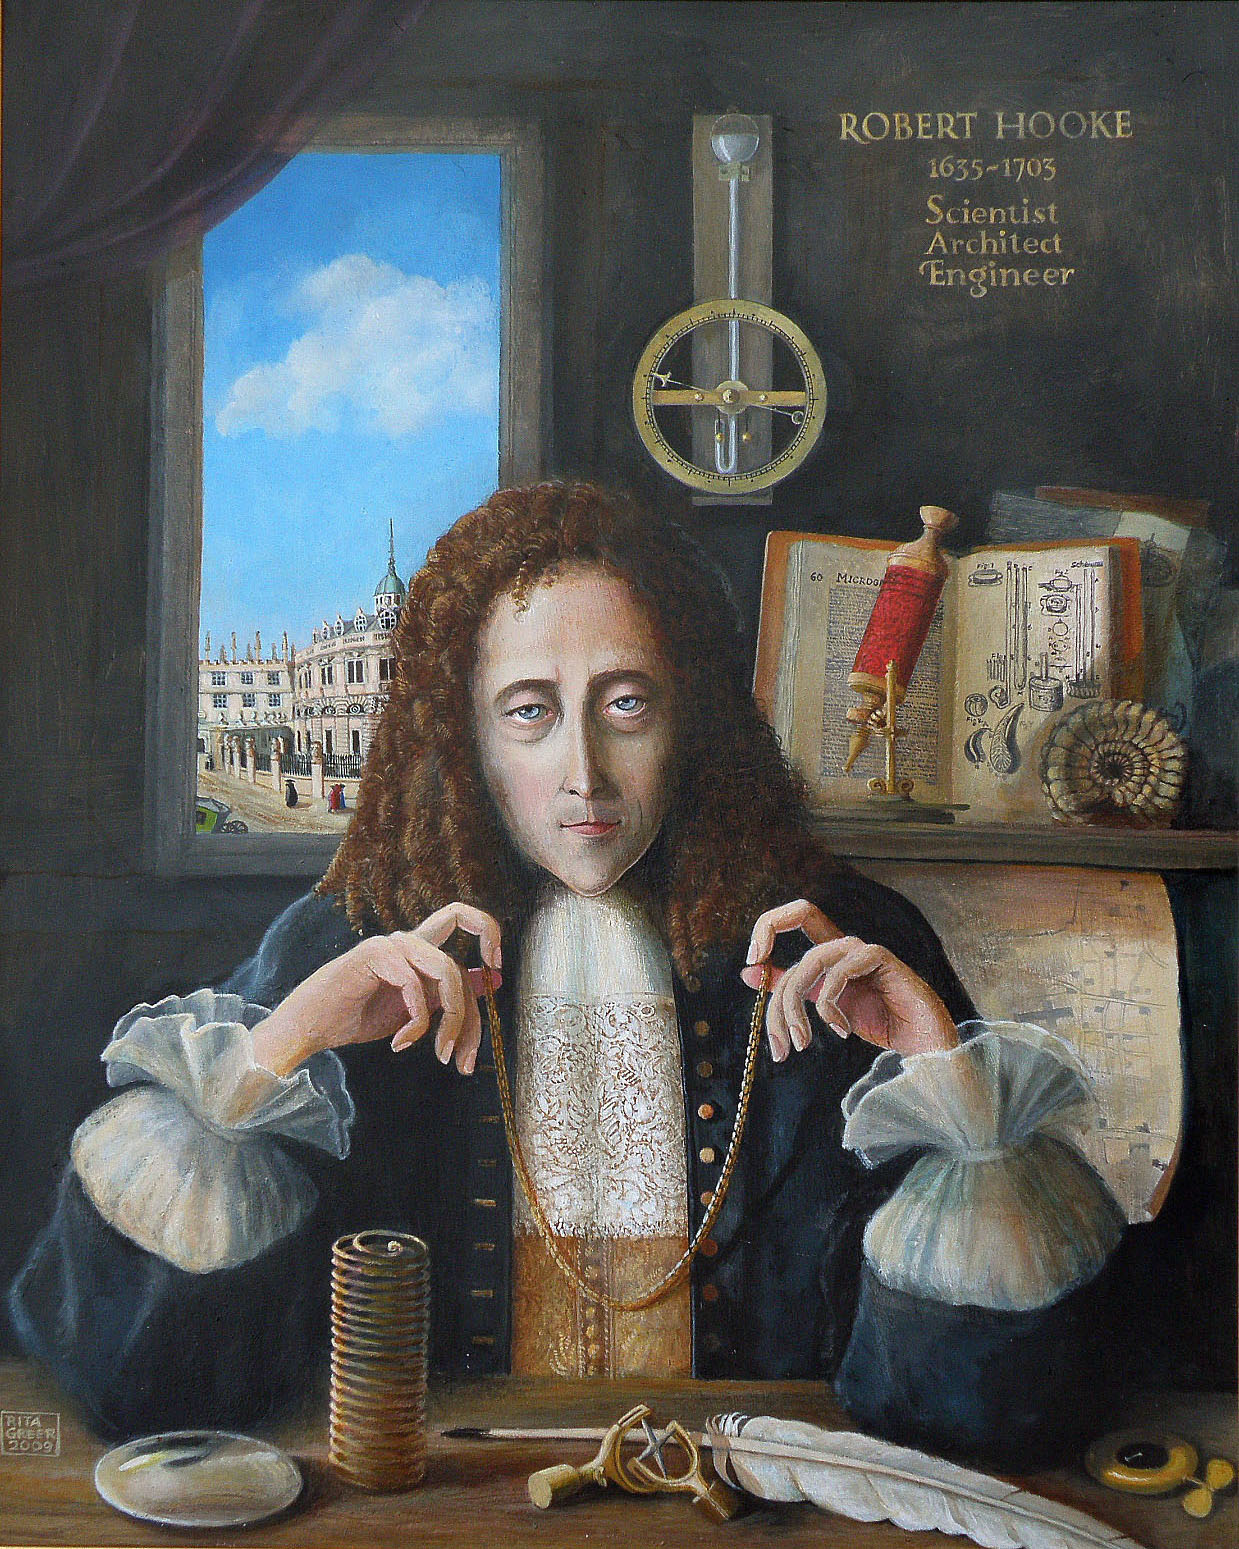
\includegraphics[width=0.7\linewidth]{revistas/002/imaxes/17_Robert_Hooke_Engineer.jpg}
    \captionof{figure}{Retrato póstumo de Robert Hooke por Rita Greer. Fonte: Wikimedia Commons}
\end{center}

\subsection*{Quen foi Robert Hooke?}

Seguro que este científico inglés non é ningún descoñecido para vós, despois de
todo, se estades nesta facultade nalgún momento tivestes que ver a famosa lei
da elasticidade que leva o seu nome: $F= -k\cdot\Delta x$. Malia que sexa a
principal razón pola que é coñecido pola maioría de nós a día de hoxe, a súa
contribución á ciencia do século XVII non foi cousa menor. Dende o seu traballo
como principal axudante nos laboratorios de Boyle ata a súa inestimable axuda á
hora de reconstruír a cidade tralo gran incendio de Londres de 1666, pasando tamén pola astronomía e a cronometría; Hooke deixou a súa pegada nas distintas áreas da ciencia e da enxeñaría do momento e ata chegou a ser nomeado presidente da Royal Society.

A súa \textit{magnum opus}, \textit{Micrographia}, supón un antes e un despois
no que a microscopía se refire, nela detállanse cincuenta e sete observacións
realizadas cun microscopio que o mesmo Hooke construíu, acompañadas por
detallados debuxos. Quizais, a achega máis destacada (e a razón pola que o
coñecerán os compañeiros e compañeiras da facultade de bioloxía) sexa que en
\textit{Micrographia} é onde se emprega por primeira vez o término ``célula''
ao describir unhas estruturas presentes nun anaco de cortizo. Esta obra, ao
estar escrita en inglés, na lingua vernácula (algo totalmente inusual para a
época), e non en latín, foi un escrito que recebiría a atención dos seus
coetáneos facilitando a accesibilidade; converteuse no primeiro \textit{best
seller} científico de todos os tempos.

\subsection*{Rivalidade con Newton}

Sereivos franco, se comecei a facer un artigo sobre a vida de Hooke non foi
polas súas múltiples achegas á ciencia, por moi interesantes e variadas que
estas fosen, senón pola continuada rivalidade que el tivo con nin máis nin
menos que Isaac Newton.

Todo comezou cando, pouco despois da publicación de \textit{Micrographia},
Newton comezou os seus propios experimentos coa luz, en concreto, o que fixo
botar chispas foi o estudo por parte de Newton do mesmo fenómeno que estudara e
describira Hooke por primeira vez na súa obra mestra. Este fenómeno trátase
dunha serie de aneis concéntricos que xorden ao pór en contacto dúas
superficies translúcidas, unha plana e outra curva.\footnote{Curiosamente, este
fenómeno coñécese como aneis de Newton, malia que non foi o primeiro en
describilos.} Isto non houbera suposto ningún problema de non ser porque Newton
en ningún momento lle deu a Hooke o crédito que este merecía por ser el o
descubridor do fenómeno. Foi así como iniciou a súa rivalidade, por unha banda,
Hooke, esixindo o crédito que merecía; pola outra, Newton, demasiado orgulloso
como para recoñecer que o seu traballo non foi totalmente orixinal. A situación
escalou durante anos, ata que a Royal Society, organización á que ambos
pertencían e da cal Hooke era presidente, veuse obrigada a intervir para evitar
que caese a reputación da mesma, polo que fixo que ambos tiveran unha
reconciliación pública. Foi neste contexto onde Newton, nunha carta a modo de
desculpa, escribe a súa tan aclamada frase <<Se puiden ver máis aló, foi porque
me encontraba sentado sobre os ombreiros duns xigantes>>.

Ben, paremos por un momento, porque isto foi o que me fixo escribir este artigo
nun primeiro lugar. Para dar contexto, Robert Hooke era un home pequeno,
corcovado e cunha deformación no lombo á raíz de diversos problemas na súa
infancia. Pois ben, disque, cando Newton escribiu a frase antes mencionada,
quixo tirar un último ataque público a Hooke, recoñece que toma o coñecemento
que achegaron os grandes sabios do pasado, eses ``xigantes'' dos que fala, pero
nunca de alguén coma Robert Hooke, quen, fisicamente, era de todo menos
xigante. Un pensaría que esta historia remataría aquí, cunha desculpa pública
de ambos e Newton tendo a última palabra, pero non, non será así.

\subsection*{Trala súa morte}

No momento en que morre Hooke, suceden dúas cousas: por unha banda, Newton
convértese en presidente da Royal Society; pola outra, publícase
\textit{Opticks}, unha extensa obra escrita por Newton sobre óptica, a cal
levaba varios anos sen publicar, agardando a morte de Hooke, para evitar
calquera posible crítica por parte deste\footnote{Newton defendía un modelo
corpuscular da luz mentres Hooke defendía o modelo ondulatorio, o que levou a
máis debates entre eles.}. Por se non for pouco, durante o cambio da sede da
Royal Society, supervisado por Newton, trasladáronse os cadros dos múltiples
presidentes que esta tivera; curiosamente, o único que nunca volveu a aparecer
foi o de Robert Hooke. Este era o único retrato que existía del, polo que non
se conserva ningunha imaxe del en vida.

Trala morte de Hooke, a súa figura como gran científico foi desaparecendo pouco
a pouco e as súas achegas fóronse minimizando ou atribuíndo a outros durante os
séculos posteriores. Non foi ata tempos relativamente recentes cando algúns
científicos e historiadores comezaron a reivindicar de novo a importancia da
súa figura na ciencia e na enxeñería, chegando a darlle o título de ``O
Leonardo da Vinci inglés''.

\begin{center}
    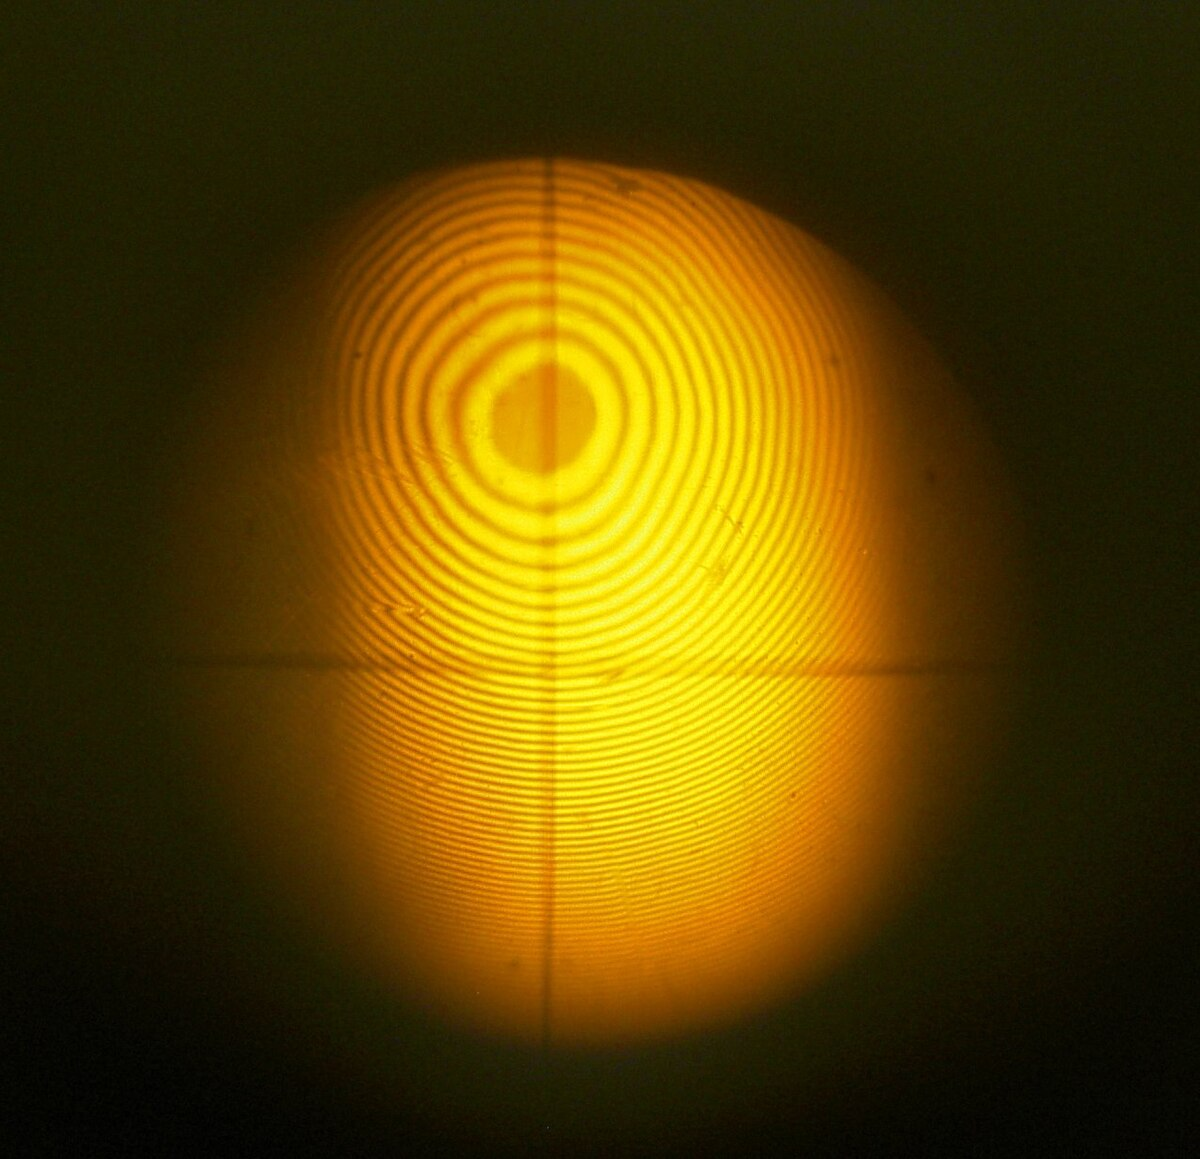
\includegraphics[scale=0.2]{revistas/002/imaxes/Newton-rings}
    \captionof{figure}{Exemplo dos \textit{aneis de Newton}. Fonte: Wikipedia}
\end{center}

\nocite{gribbin2004historia}
\printbibliography

\end{multicols}
\end{refsection}
